\documentclass[12pt,a4paper]{article}

\usepackage[T1]{fontenc}
\usepackage[utf8]{inputenc}
\usepackage[margin=2.5cm]{geometry}
\usepackage{graphicx}
\usepackage[hidelinks]{hyperref}
\usepackage{fancyhdr}
\usepackage{lastpage}
\usepackage{appendix}
\usepackage{amsmath}
\usepackage{mathtools}
\usepackage{color}
\usepackage{palatino}
\usepackage[strict]{changepage}
\usepackage{subcaption}
\usepackage{enumitem}
\usepackage{csquotes}
\usepackage{verbatim}
\usepackage[cache=false]{minted}
\usepackage[ruled,vlined]{algorithm2e}

\newenvironment{changemargin}[2]{%
  \begin{list}{}{%
      \setlength{\topsep}{0pt}%
      \setlength{\leftmargin}{#1}%
      \setlength{\rightmargin}{#2}%
      \setlength{\listparindent}{\parindent}%
      \setlength{\itemindent}{\parindent}%
      \setlength{\parsep}{\parskip}%
    }%
  \item[]}{\end{list}}

\DeclarePairedDelimiter\ceil{\lceil}{\rceil}
\DeclarePairedDelimiter\floor{\lfloor}{\rfloor}

\usemintedstyle{default}
\setminted{
  linenos=true,
  breaklines=true,
  fontsize=\small,
  frame=single,
}

\title{Community detection in networks}
\author{Carlos Requena López}

%% Fancy layout
\pagestyle{fancy}
\lhead{INFO-F521}
\chead{}
\rhead{}
\lfoot{}
\cfoot{}
\rfoot{Page \thepage\ of \pageref{LastPage}}
\renewcommand{\headrulewidth}{0.4pt}
\renewcommand{\footrulewidth}{0.4pt}


%%% --- %%% --- DOCUMENT START --- %%% --- %%%
\begin{document}
\thispagestyle{fancy}
\maketitle
\thispagestyle{fancy}

\section{Introduction}

The topic of this assignment is community detection in networks by
means of hierarchical clustering. Informally, network communities can
be seen as dense (highly connected) subgraphs that are connected
between each other sparsely, only by few arcs or edges.

Hierarchical clustering (HC) refers to the technique of grouping
together elements that share some sort of similarity and separating
those that do not. HC can be \emph{divisive}, where elements start in
one cluster and are removed gradually or \emph{agglomerative}, where
every unit is its own cluster and are merged step by step. Only
\emph{agglomerative} clustering will be considered in this assignment:
in particular single-linkage and complete-linkage clustering.

\section{Analysis and expectations}

\subsection{Measure of similarity}

Let $ G = (V, E) $ be a simple, unweighted, undirected graph. Let $A$
be the adjacency matrix of $G$, defined as follows:

\[
  A_{ij} =
  \begin{cases}
    1 & \quad \text{if } (i,j) \in E\\
    0 & \quad \text{otherwise }
  \end{cases}
\]

We will use this adjacency matrix as the only source of information to
determine the similarity between vertices in the graph, but there
could be plenty of other sources depending on the application
domain. For example, when analysing text files, the similarity measure
could be the amount of equal significant words each one contains, or
in the case of aminoacids, the number of appearances at a certain
location.

Here, however, we compute the mean and variance between the rows of
the adjacency matrix as follows (if $A$ was not symmetric or $G$
undirected, it would have to be computed for rows \emph{and} columns):

$$ \mu_i = \frac{1}{n} \sum_{j=1}^{n} A_{ij} $$

$$ \sigma^2 = \frac{1}{n} \sum_{j=1}^{n} (A_{ij} - \mu_i)^2 $$

The similarity measure in this case is the Pearson product-moment
correlation coefficient:

$$ x_{ij} = \frac{\frac{1}{n}\sum_{k=1}^{n}(A_{ik} -
  \mu_i)(A_{jk}-\mu_j)}{\sigma_i\sigma_j} $$

All diagonal elements are excluded from these calculations
\cite[p.~369]{socionetwork}. The value $x_{ij}$ can range from -1 to
1, and it gives a measure of how structurally similar two vertices
are. Two vertices do not need to be adjacent for this quantity to be
significant, although they usually are.

\subsection{Hierarchical clustering}

Once the similarity measures are set, they serve as a base to
implement agglomerative HC. By observing the set of partitions (the
number of partitions is the number of elements at step 0), we can
define the function to maximise when merging two of them. This is
repeated until there is only one partition (containing all the
elements) left.

Algorithms for HC do not require the size of the partitions of the
number of partitions to be specified. Obviously, the output of the
program - a set containing all vertices - is not really meaningful;
that is why the process is captured in a data structure called
\emph{dendogram}. This one can be \emph{cut} horizontally to inspect
the clusters at the cut level.

\subsubsection{Pseudocode of single linkage and complete linkage
  algorithms}

The pseudocodes for basic single linkage and complete linkage
clustering are given in algorithms \ref{slink} and \ref{clink}.

\begin{algorithm}[h]
  \SetAlgoLined
  \KwIn{An undirected graph G}
  \KwOut{The tree of clusters}

  \nl Compute the proximity (similarity) matrix X for the given G.\;
  \nl Place every vertex in its own set.\;
  \nl Find the two most similar elements in different sets and merge them.\;
  \nl Remove one of the entries in X and update the other by choosing the highest
  values possible.\;
  \nl Append merge information to tree to keep the history of events.\;
  \nl \While{X \textrm{has shape} > 1x1}{
    \nl Repeat lines 3 through 5\;
  }
  \caption{\bf SLOW\_S-LINK}
  \label{slink}
\end{algorithm}

\begin{algorithm}[h]
  \SetAlgoLined
  \KwIn{An undirected graph G}
  \KwOut{The tree of clusters}

  \nl Compute the proximity (similarity) matrix X for the given G.\;
  \nl Place every vertex in its own set.\;
  \nl Find the two most similar elements in different sets and merge them.\;
  \nl Remove one of the entries in X and update the other one by choosing the lowest
  values possible.\;
  \nl Append merge information to tree to keep the history of events.\;
  \nl \While{X \textrm{has shape} > 1x1}{
    \nl Repeat lines 3 through 5\;
  }
  \caption{\bf SLOW\_C-LINK}
  \label{clink}
\end{algorithm}

The last step of the algorithm, which is keeping information about
the merges done, is useful to plot the dendogram or recreate the
merge history and be able to ``cut'' the tree at a certain point to
obtain the partitions.

\subsubsection{Computational complexity}

For both cases, the complexity of the algorithm is
$\mathcal{O}(n^3)$: computing the similarity matrix (or distance
information) takes $\mathcal{O}(nm)$ \cite{newman}, where $n$ is the
number of vertices and $m$ is the number of edges. We need to check
the minimum element in an array of size $n^2$, so by the adversary
argument, this takes $\Omega (n^2)$, and this check has to be
done a maximum of $n$ times. Therefore, the upper bound for the
naive algorithm is $\mathcal{O}(n^3)$.

As a side note, the library \texttt{SciPy} for Python, implements an
$\mathcal{O}(n^2)$ algorithm for single-linkage and
complete-linkage, based on minimum spanning tree and
nearest-neighbour chain respectively.

\subsubsection{Differences between single link and complete link}

On the one hand, single-linkage merges two clusters or partitions by
retaining the maximum similarity (or minimum distance) between the
two. The main formula behind the concept of single linkage is:

$$ \mathrm{max}\{x_{i,j} : i \in P_a, j \in P_b\} $$

where ${P_a}$ and $P_b$ are two partitions of $V$.

This gives rise to the \emph{chaining phenomenon}, e.g.: if
there is a very ``powerful'' node with high similarity with a lot of
other nodes, the latter will be chained successively to the first
one since it is the only one that counts in that cluster.

On the other hand, complete linkage remembers the ``weakest'' or more
distant element there is when merging two clusters. This results in
more balanced, similar sized clusters. Usually, this is what we are
looking for. The function used is:

$$ \mathrm{min}\{x_{i,j} : i \in P_a, j \in P_b\} $$

The main disadvantage of complete linkage is that it considers
degenerate points (isolated vertices in our case) to have more
importance than what they really do.

A third approach not discussed here, \emph{average linkage}, does not
consider a single vertex (the one with lowest or highest scores) per
partition. Instead, it computes an average of similarities among the
members of the newly created partition, and sets the score of the
member to that average.

Figures \ref{fig:slink-vs-clink} and \ref{fig:slink-vs-clink2} show an
example for the same random graph, for single-linkage and
complete-linkage at two different cuts in the tree.

\begin{figure}
  \centering
  \begin{subfigure}[h]{0.49\textwidth}
    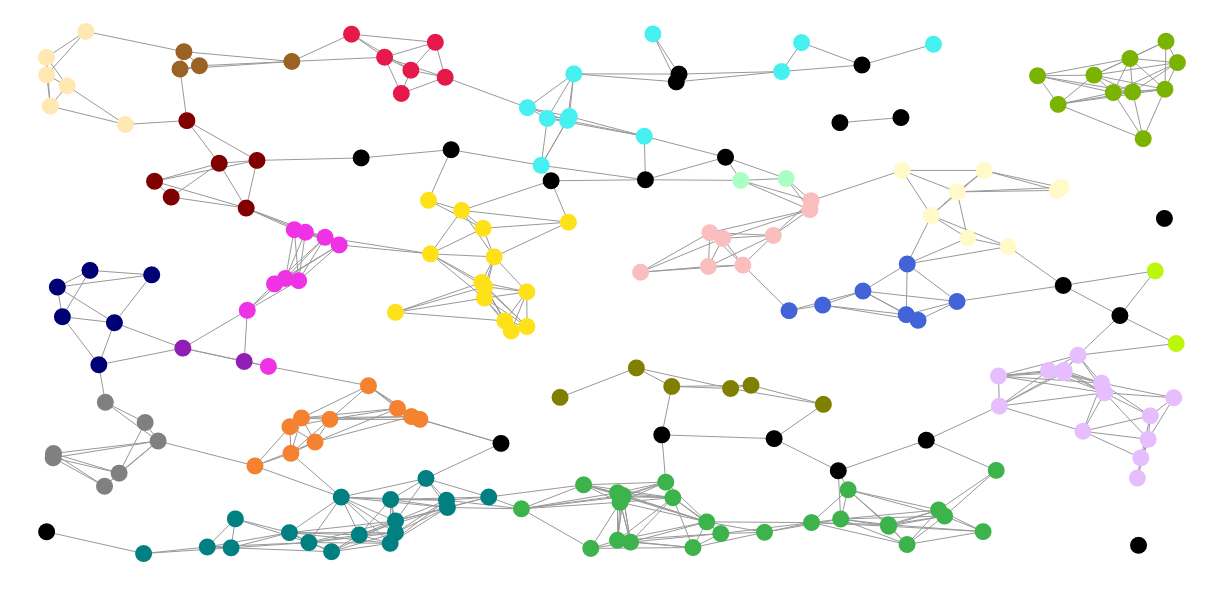
\includegraphics[width=\linewidth]{img/slink-200-160.png}
    \caption{Single linkage}
  \end{subfigure}
  \begin{subfigure}[h]{0.49\textwidth}
    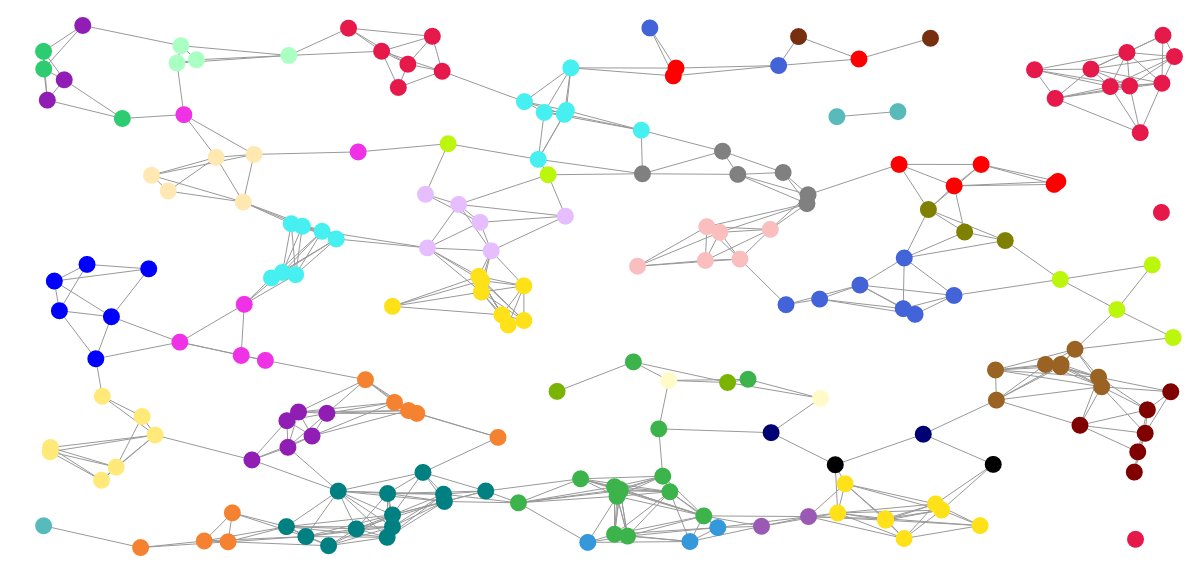
\includegraphics[width=\linewidth]{img/clink-200-160.png}
    \caption{Complete linkage}
  \end{subfigure}
  \caption{Random graph. Tree cut at step 160. For $n = 200$}
  \label{fig:slink-vs-clink}
\end{figure}

\begin{figure}
  \centering
  \begin{subfigure}[h]{0.49\textwidth}
    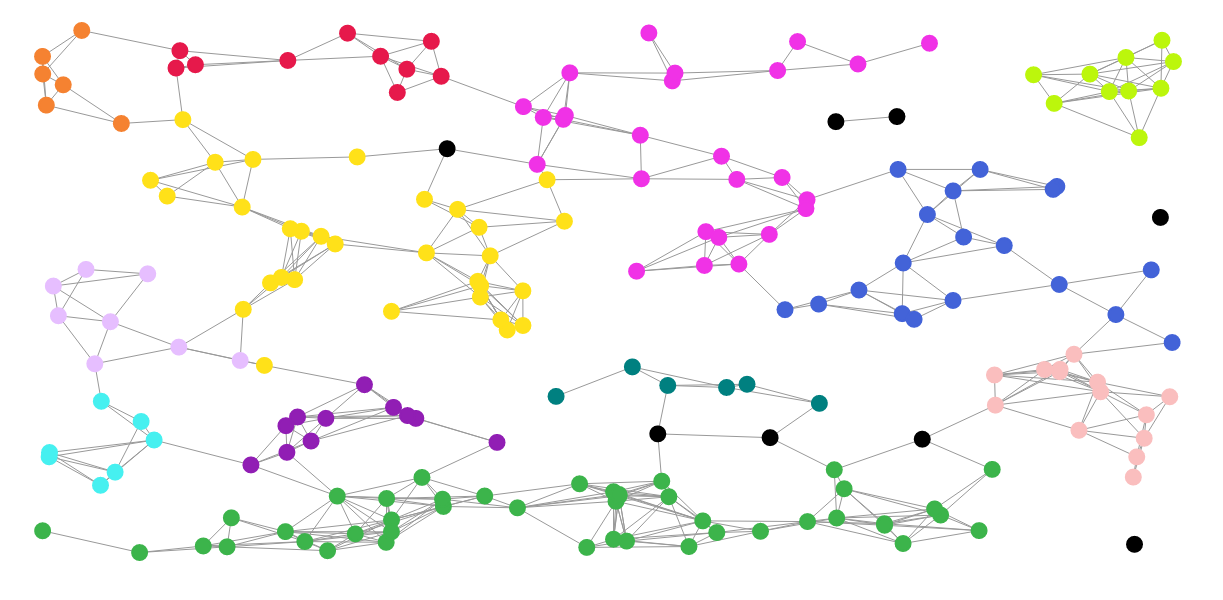
\includegraphics[width=\linewidth]{img/slink-200-180.png}
    \caption{Single linkage}
  \end{subfigure}
  \begin{subfigure}[h]{0.49\textwidth}
    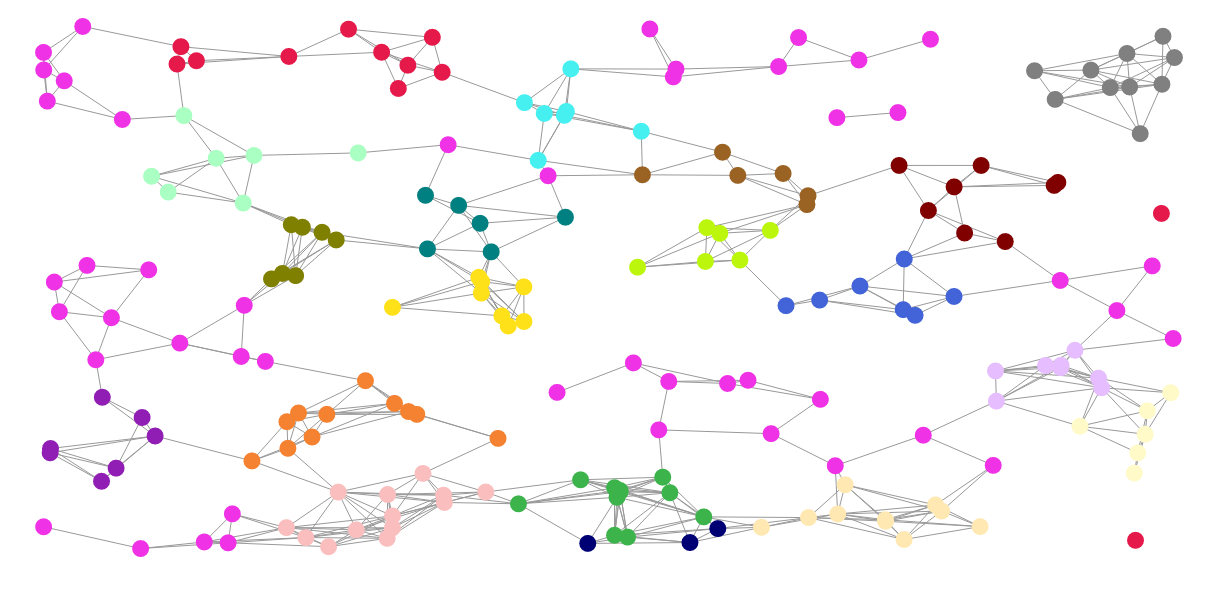
\includegraphics[width=\linewidth]{img/clink-200-180.png}
    \caption{Complete linkage}
  \end{subfigure}
  \caption{Random graph. Tree cut at step 180. For $n = 200$}
  \label{fig:slink-vs-clink2}
\end{figure}

Every colour represents a different partition.

\subsubsection{Optimality of solution at each step}

For single-linkage, we define a partitioning to be optimal if the
quantity:

$$ \sum_{C_1, C_2 \in \mathcal{P}} \mathrm{max}(Sim(C_1, C_2)) $$

is minimum for all possible partions with the same number of
classes. This means the separation between classes is maximum.

To simplify things, let's consider clustering with euclidean distances
(instead of similarity based on the structural properties of a
graph). One such partitioning is shown in figure \ref{fig:simple}. In
this example, there are 3 classes, coloured with red, blue and
green. The claim is that this is the best possible partitioning and it
is chosen by single linkage.

\begin{figure}[ht!]
  \centering
  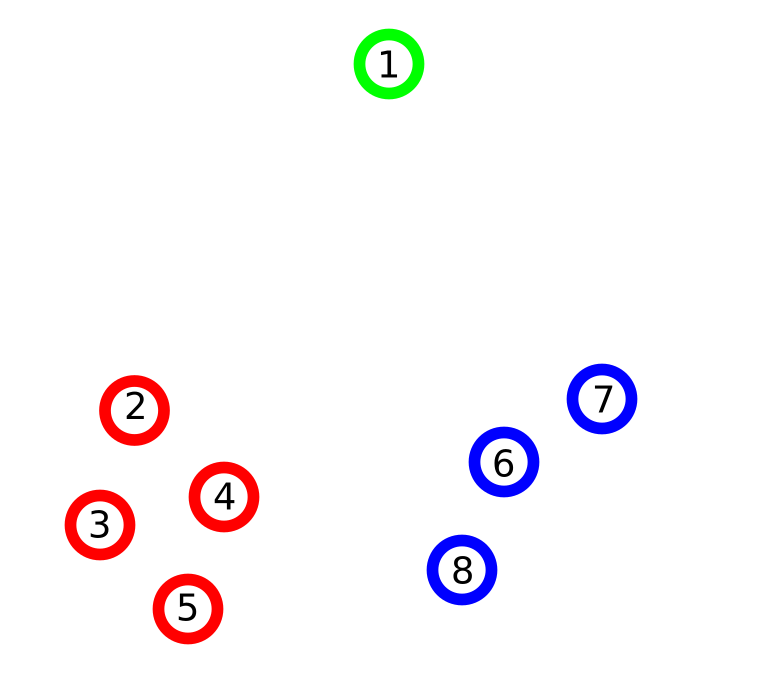
\includegraphics[width=0.5\textwidth]{img/simple.png}
  \caption{A possible 3-class partitioning for 8 points in the plane}
  \label{fig:simple}
\end{figure}

In figure \ref{fig:simple}, the sum of the shortest distance (maximum
similarity) between classes is given by: $d(1,2) + d(1, 7) + d(4,8)$
and it is the maximum total distance (minimal total similarity) we can
get. Swapping the colour of any element to obtain a different
partitioning would give a smaller quantity.

Let's suppose 1 is swapped with 2, making the number smaller. Is this
a possible scenario for single linkage ? It isn't, since, by choosing
the maximum similarity couple at every step, the total between classes
remains the minimum. Point 1 would have chosen point 2 before 3 or 4.

We can also think of single-linkage as building a minimum
spanning-tree. If there was some path of smaller distance that was not
chosen, the spanning-tree built would not be minimum.

The same can be said about complete-linkage and maximising the total
maximum distance (minimum similarity) between classes, since out of
the list of long distances, we are taking the minimum one, and then
updating so the maximum distances are kept, yielding maximum distances
in general.


\subsubsection{What happens in the case of a tie?}

If at step $s$, there are 4 classes $C_1, C_2, C_3, C_4$ of a given
possible partition, such that:

$$ Sim(C_1, C_2) = Sim(C_3, C_4) = \max_{C_i, C_j \in
  \mathcal{P}_s}(Sim(C_i, C_j))\ \ \ \ \ \ (\mathrm{Figure}\
\ref{fig:tie-single})  $$

\begin{itemize}
\item Choosing to merge $C_1$ and $C_2$ we obtain
  $\mathcal{P}_{s+1}^{A}$
\item Choosing to merge $C_3$ and $C_4$ we obtain
  $\mathcal{P}_{s+1}^{B}$
\end{itemize}

In both cases $\mathcal{P}_{s+2}$ will be the same. The partition that
wasn't merged, will be merged. In the case of single linkage, no other
couple can appear at $s+1$ with a bigger similarity than what we have
at step $s$. In the case of complete linkage, even less so, since we
update similarities taking the less similar elements.

Figure \ref{fig:tie-single} shows the analogy to euclidean distances
in the plane, since they are easier to visualise than the computed
Pearson correlation for graphs. A tie would mean 3 or more points, all
equidistant from each other. On this figure, classes $C_1$ and $C_2$
are at the same distance as classes $C_3$ and $C_4$.

\begin{figure}[ht!]
  \centering
  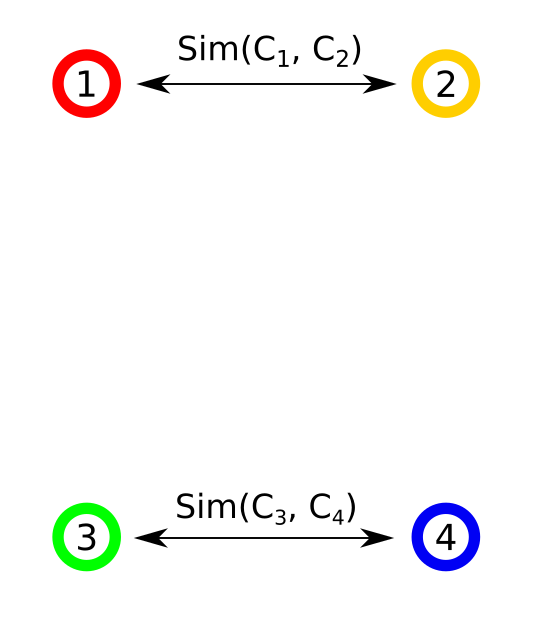
\includegraphics[width=0.5\textwidth]{img/tie.png}
  \caption{Tie with 4 classes}
  \label{fig:tie4}
\end{figure}

Nonetheless a different thing happens if the tie occurs between a
triplet of elements:

$$ Sim(C_1, C_2) = Sim(C_1, C_3) = \max_{C_i, C_j \in
  \mathcal{P}_s}(Sim(C_i, C_j))\ \ \ \ \ \ (\mathrm{Figure}\
\ref{fig:real-tie})  $$

\begin{figure}[ht!]
  \centering
  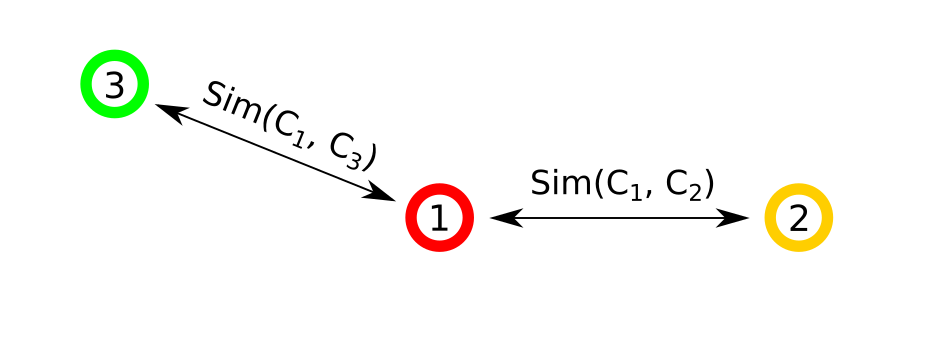
\includegraphics[width=0.8\textwidth]{img/real-tie.png}
  \caption{Tie with 3 classes}
  \label{fig:real-tie}
\end{figure}

In this case, using single linkage and merging $C_1$ and either one of
$C_2$ or $C_3$ first, the unmerged element still retains the maximum
similarity with this newly created class (although more ties could
appear).

However, using complete linkage, if $C_1$ and $C_2$ are to be merged,
$C_3$ might lose its status of maximum similarity with this new
cluster. The partition $\mathcal{P}_{s+2}^A$ and in general
$\mathcal{P}_{s+i}^{A}$ for the $i$ successive steps could look very
different from $\mathcal{P}_{s+i}^B$.

We therefore sometimes say that single-linkage is \emph{insensitive}
to ties.

As a side note, several approaches exist to deal with the
non-uniqueness problem of similarities in the data set and are
described in \cite{nonunique}:

\begin{itemize}
\item Arbitrarily choosing between the elements in the tie.
\item Deterministically choosing between the elements in the tie
  (the element with smaller index for example).
\item Merge all tied elements at the same time.
\end{itemize}


\section{Implementation and results}

Several tests on random geometric graph with different parameters can
be run to verify how both methods perform. The tree will be cut at a
late stage, in order to obtain decently sized clusters. We can then
check if the clusters correspond to dense areas of the graph that have
sparse connections to other components.

The test network places $n$ vertices uniformly at random on a one by
one canvas, and traces an edge from on to another if their distance is
at most a radius $r$. This type of network can easily mimic
communities and is useful to test clustering.

\begin{figure}
  \centering
  \begin{subfigure}[h]{0.8\textwidth}
    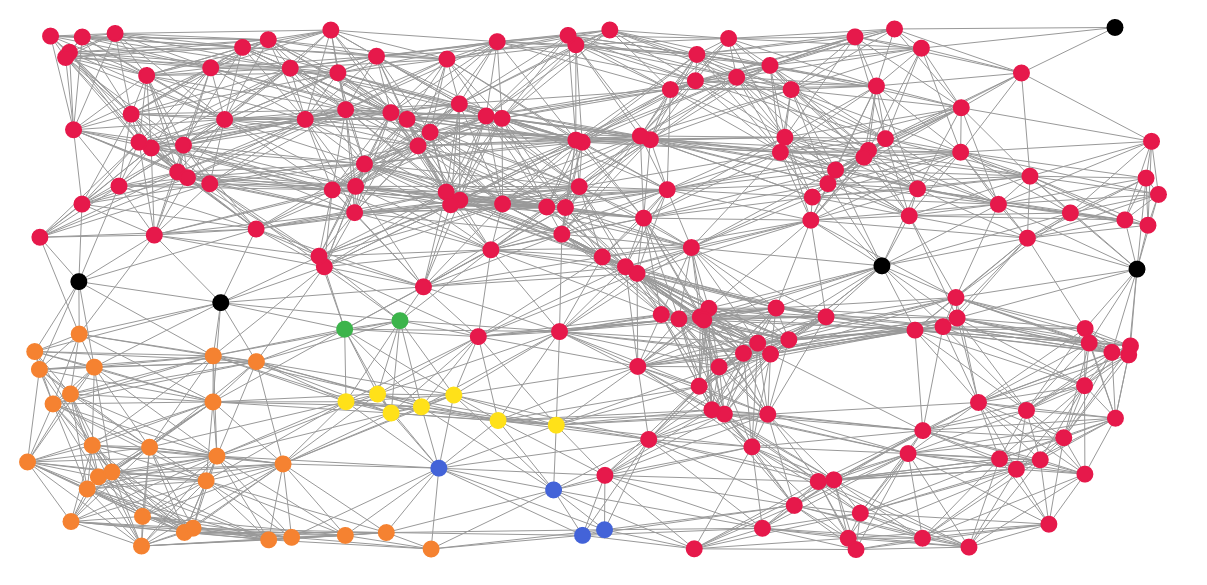
\includegraphics[width=\linewidth]{img/slink-200-170-02.png}
    \caption{Single linkage}
  \end{subfigure}
  \begin{subfigure}[h]{0.8\textwidth}
    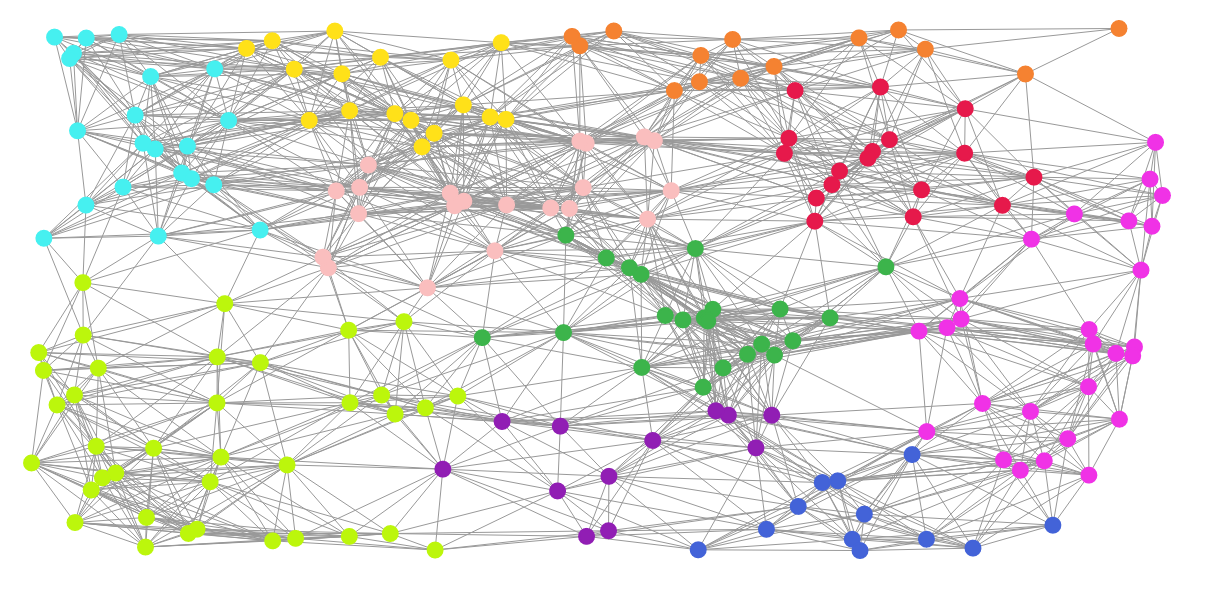
\includegraphics[width=\linewidth]{img/clink-200-170-02.png}
    \caption{Complete linkage}
  \end{subfigure}
  \caption{Random graph. $n = 200$. $r = 0.2$. Cut at step 170}
  \label{fig:170-0.2}
\end{figure}

\begin{figure}
  \centering
  \begin{subfigure}[h]{0.8\textwidth}
    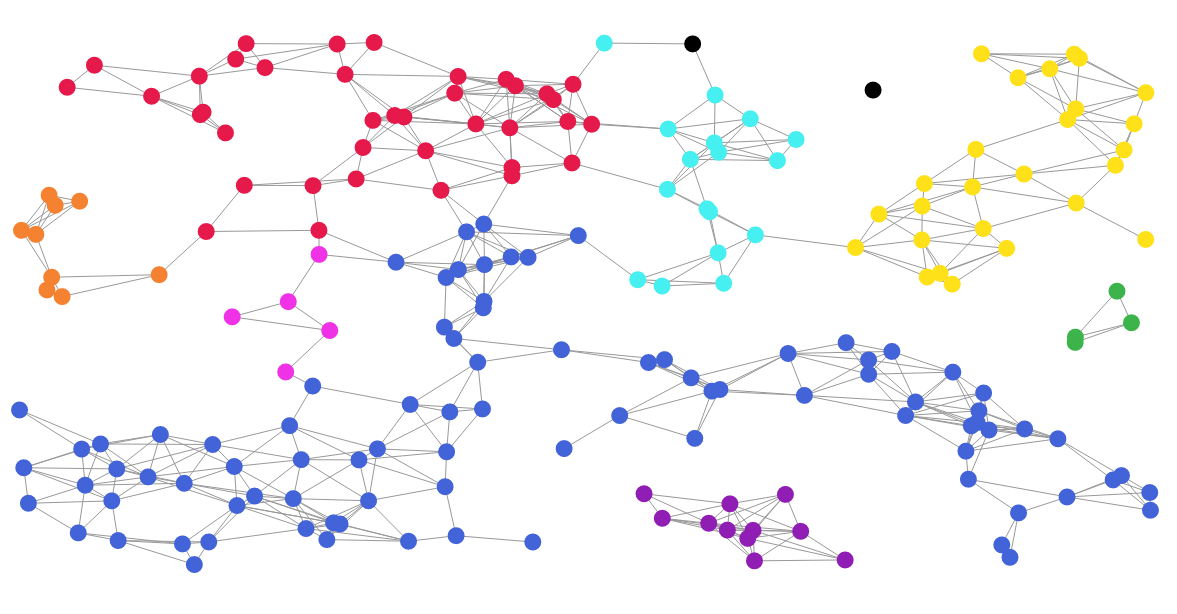
\includegraphics[width=\linewidth]{img/slink-200-170-01.png}
    \caption{Single linkage}
  \end{subfigure}
  \begin{subfigure}[h]{0.8\textwidth}
    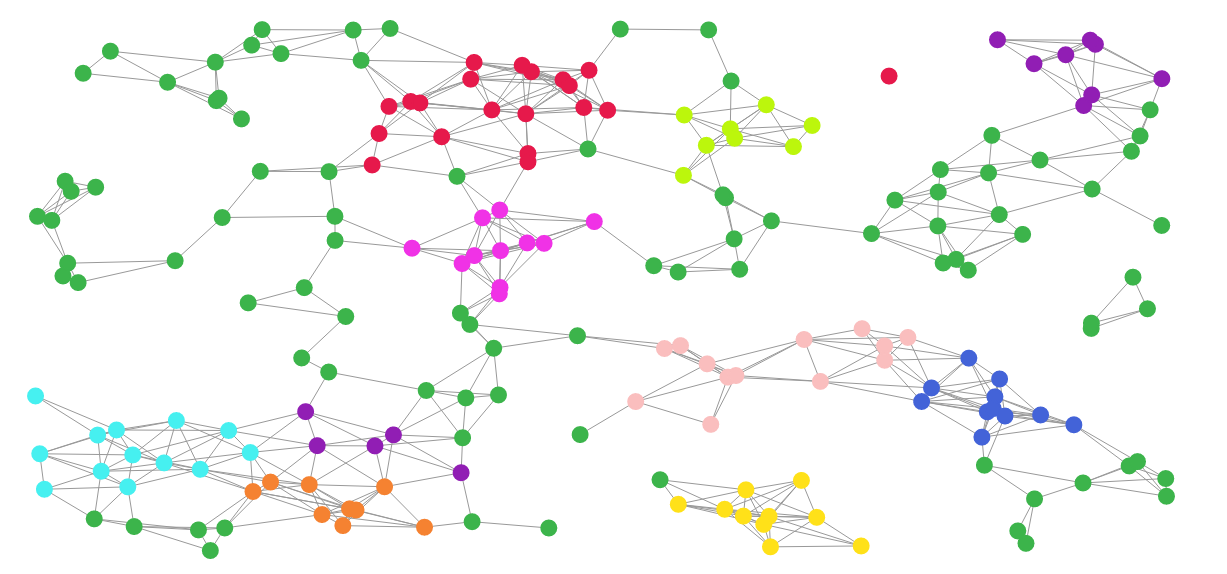
\includegraphics[width=\linewidth]{img/clink-200-170-01.png}
    \caption{Complete linkage}
  \end{subfigure}
  \caption{Random graph. $n = 200$. $r = 0.1$. Cut at step 170}
  \label{fig:170-0.1}
\end{figure}

\begin{figure}
  \centering
  \begin{subfigure}[h]{1\textwidth}
    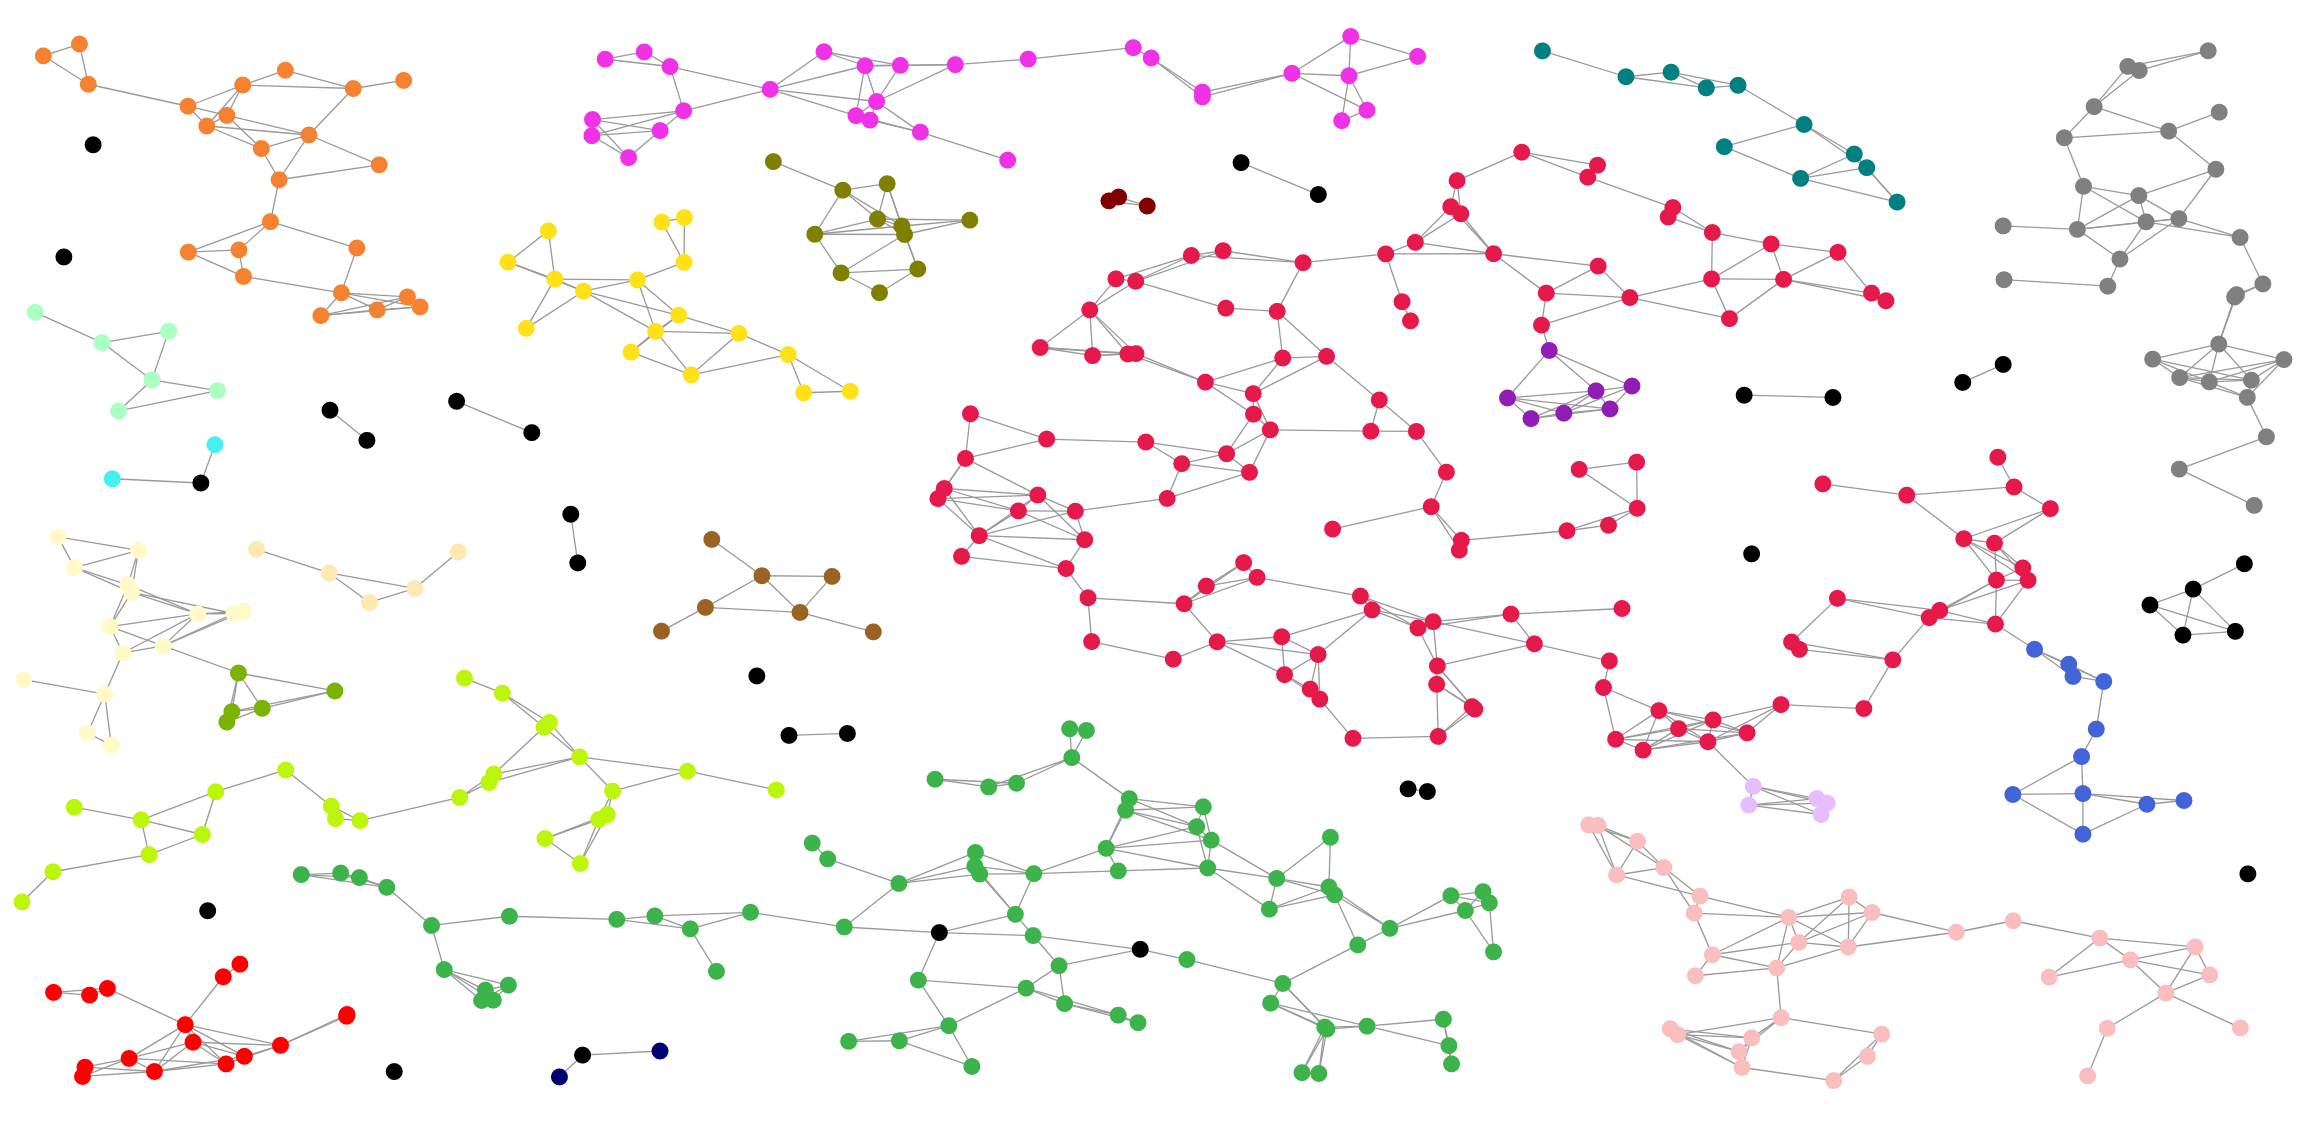
\includegraphics[width=\linewidth]{img/slink-500-450-005.png}
    \caption{Single linkage}
  \end{subfigure}
  \begin{subfigure}[h]{1\textwidth}
    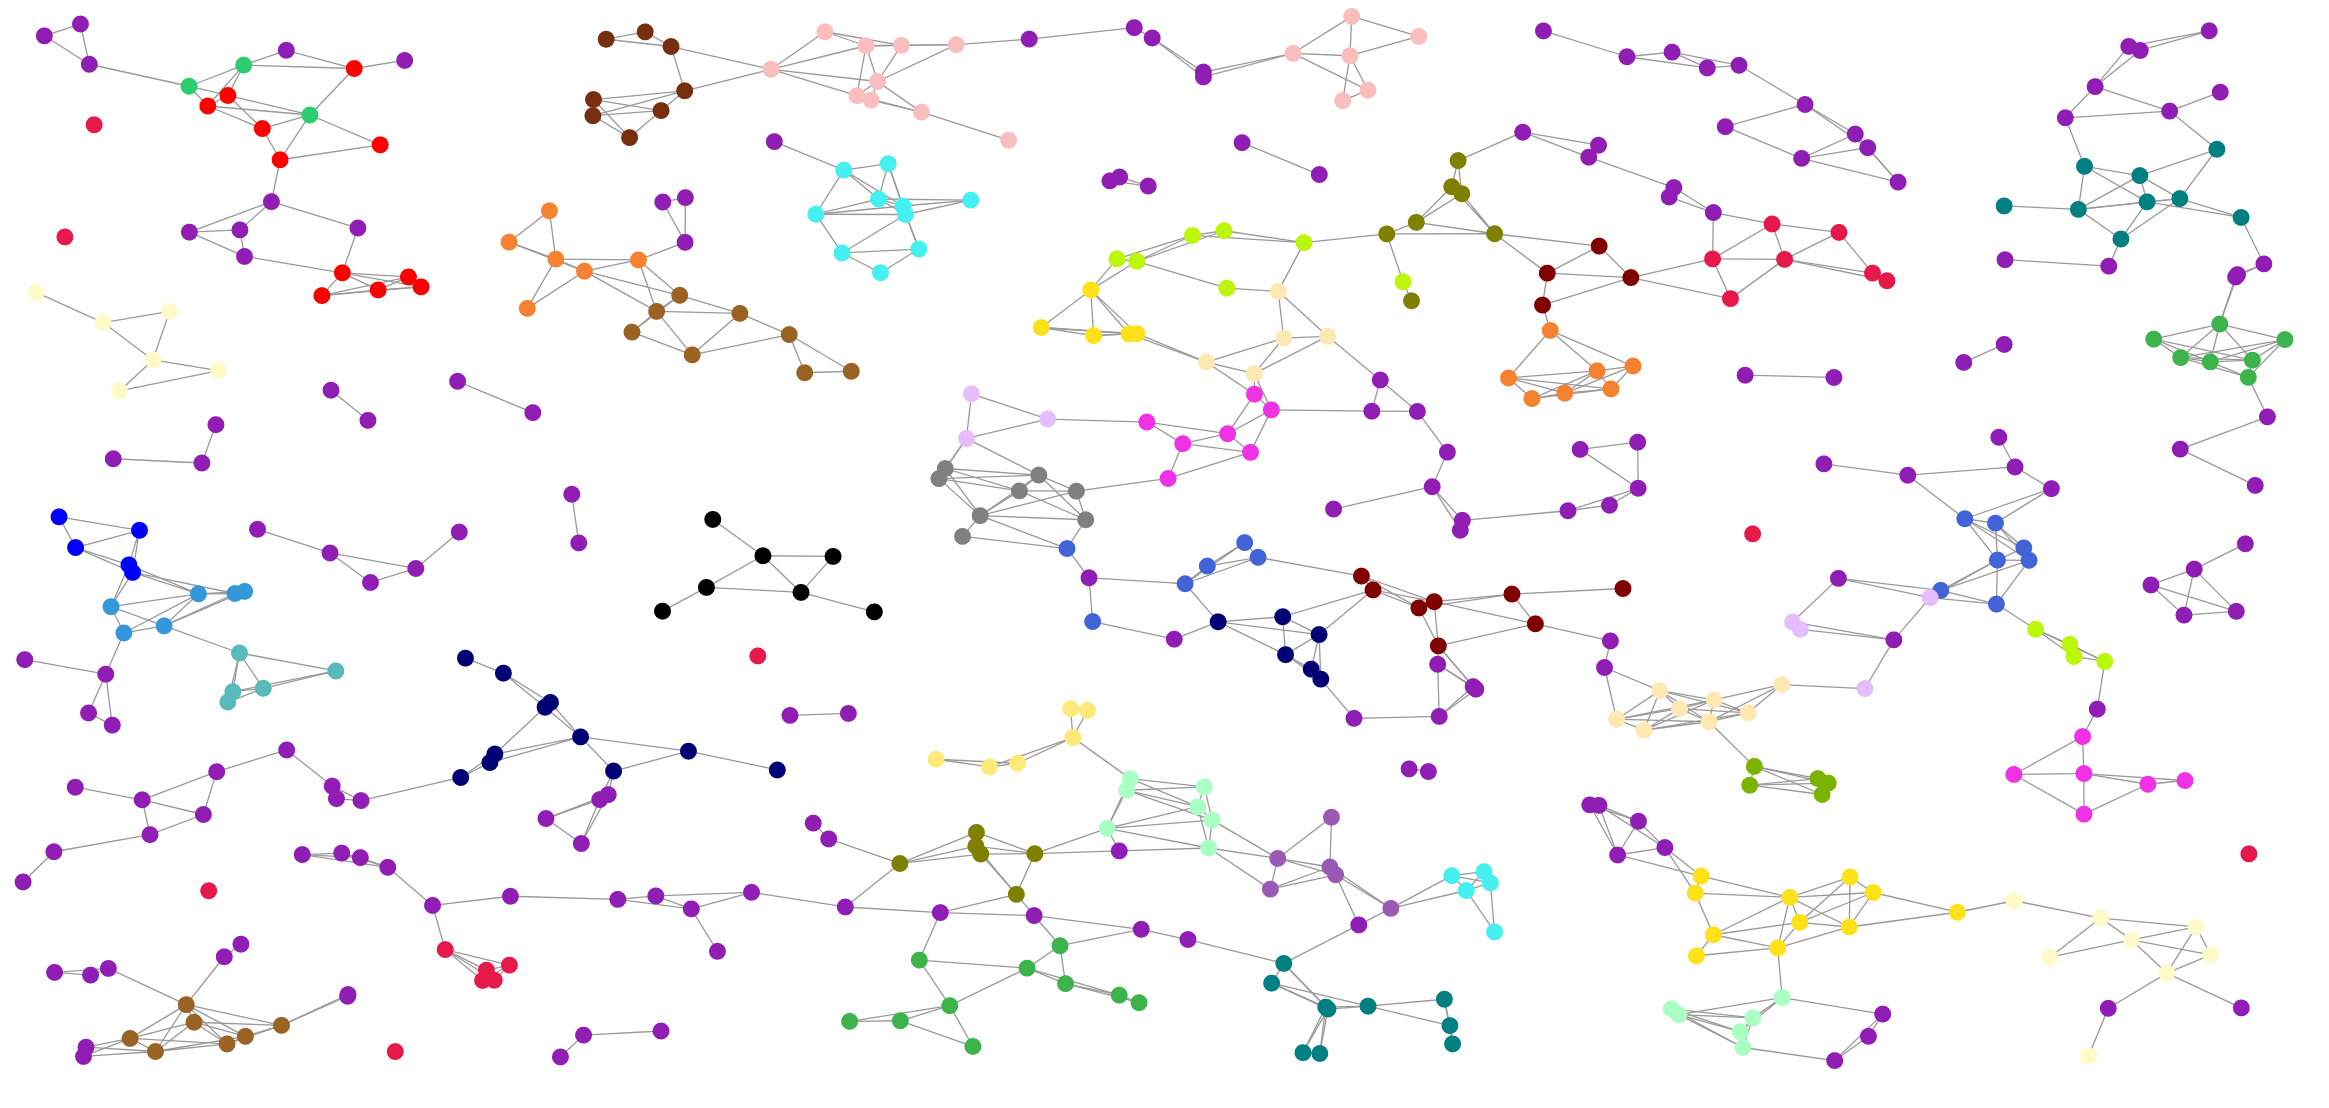
\includegraphics[width=\linewidth]{img/clink-500-450-005.png}
    \caption{Complete linkage}
  \end{subfigure}
  \caption{Random graph. $n = 500$. $r = 0.05$. Cut at step 450}
  \label{fig:450-0.05}
\end{figure}

\section{Conclusion}

These naive implementations of single-linkage and complete-linkage
hierarchical clustering perform well on a different range of cases.

In Figure \ref{fig:170-0.2}, the chaining phenomenon can be
appreciated. At the same cut level, single linkage has a bloated class
while complete linkage tries to keep balanced classes.

In general, complete-linkage tends to merge vertices that do not form
part of the same community on sparse graphs, such as in Figures
\ref{fig:170-0.1} and \ref{fig:450-0.05}, but works better on later
stages in dense graphs (Figure \ref{fig:170-0.2}).

Single linkage does also perform very well putting disconnected
components in their own cluster, or even components with a few bridges
to other components, as can be seen in Figure \ref{fig:170-0.1}.

\bibliographystyle{ieeetr}
\bibliography{main}
\nocite{*}

\appendix
\section{Appendix - code listing}

\inputminted[label=main.py]{python}{../src/main.py}
\hfill
\inputminted[label=measures.py]{python}{../src/measures.py}
\hfill
\inputminted[label=clink.py]{python}{../src/link.py}

\end{document}
